% File SDSS2020_SampleExtendedAbstract.tex
\documentclass[10pt]{article}\usepackage[]{graphicx}\usepackage[]{color}
% maxwidth is the original width if it is less than linewidth
% otherwise use linewidth (to make sure the graphics do not exceed the margin)
\makeatletter
\def\maxwidth{ %
  \ifdim\Gin@nat@width>\linewidth
    \linewidth
  \else
    \Gin@nat@width
  \fi
}
\makeatother

\definecolor{fgcolor}{rgb}{0.345, 0.345, 0.345}
\newcommand{\hlnum}[1]{\textcolor[rgb]{0.686,0.059,0.569}{#1}}%
\newcommand{\hlstr}[1]{\textcolor[rgb]{0.192,0.494,0.8}{#1}}%
\newcommand{\hlcom}[1]{\textcolor[rgb]{0.678,0.584,0.686}{\textit{#1}}}%
\newcommand{\hlopt}[1]{\textcolor[rgb]{0,0,0}{#1}}%
\newcommand{\hlstd}[1]{\textcolor[rgb]{0.345,0.345,0.345}{#1}}%
\newcommand{\hlkwa}[1]{\textcolor[rgb]{0.161,0.373,0.58}{\textbf{#1}}}%
\newcommand{\hlkwb}[1]{\textcolor[rgb]{0.69,0.353,0.396}{#1}}%
\newcommand{\hlkwc}[1]{\textcolor[rgb]{0.333,0.667,0.333}{#1}}%
\newcommand{\hlkwd}[1]{\textcolor[rgb]{0.737,0.353,0.396}{\textbf{#1}}}%
\let\hlipl\hlkwb

\usepackage{framed}
\makeatletter
\newenvironment{kframe}{%
 \def\at@end@of@kframe{}%
 \ifinner\ifhmode%
  \def\at@end@of@kframe{\end{minipage}}%
  \begin{minipage}{\columnwidth}%
 \fi\fi%
 \def\FrameCommand##1{\hskip\@totalleftmargin \hskip-\fboxsep
 \colorbox{shadecolor}{##1}\hskip-\fboxsep
     % There is no \\@totalrightmargin, so:
     \hskip-\linewidth \hskip-\@totalleftmargin \hskip\columnwidth}%
 \MakeFramed {\advance\hsize-\width
   \@totalleftmargin\z@ \linewidth\hsize
   \@setminipage}}%
 {\par\unskip\endMakeFramed%
 \at@end@of@kframe}
\makeatother

\definecolor{shadecolor}{rgb}{.97, .97, .97}
\definecolor{messagecolor}{rgb}{0, 0, 0}
\definecolor{warningcolor}{rgb}{1, 0, 1}
\definecolor{errorcolor}{rgb}{1, 0, 0}
\newenvironment{knitrout}{}{} % an empty environment to be redefined in TeX

\usepackage{alltt}
\usepackage{newtxtext, newtxmath, times}
\usepackage{sdss2020} % Uses Times Roman font (either newtx or times package)
\usepackage{url}
\usepackage{latexsym}
\usepackage{amsmath, amsfonts}
\usepackage{algorithm, algorithmic}  
\usepackage{graphicx}

%\title{Symposium on Data Science and Statistics (SDSS 2022) \\
%Submission and Formatting Instructions for Extended Abstracts}

\title{Exploring Rural Shrink Smart Through Guided Discovery Dashboards}

\author{
  Denise Bradford \\
  University of Nebraska - Lincoln \\
  Lincoln, Nebraska \\
  {\tt denise.bradford@huskers.unl.edu} \\\And
  Susan VanderPlas \\
  University of Nebraska - Lincoln \\
  Lincoln, Nebraska \\
  {\tt susan.vanderplas@unl.edu} \\}
  

\date{}
\IfFileExists{upquote.sty}{\usepackage{upquote}}{}
\begin{document}




\maketitle
\begin{abstract}
Many small and rural places are shrinking. Interactive dashboards are the most common use cases for data visualization and context for exploratory data tools. In our paper, we will explore the specific scope of how dashboards are used in small and rural area to empower novice analysts to make data-driven decisions. Our framework will suggest a number of research directions to better support small and rural places from shrinking using an interactive dashboard design, implementation and use for the every day analyst. 
\end{abstract}

{\bf Keywords:} Interactive Dashboards, Exploratory Data Analysis (EDA), Guided Discovery

\section{Research Problem}
With the amount of publicly open-source data, a proliferation of visualization dashboards has increased in nearly every industry \cite{fisher}. A dashboard in its fundamental form, a dashboard supports a way of presenting and making sense of complex data to better enable and support decision making. Stephen Few defines a dashboard as:

\begin{quotation}
\small A visual display of the most important information needed to achieve one or more objectives, consolidated and arranged on a single screen so the information can be monitored at a glance. \cite{few}
\end{quotation}

Some communities continue to thrive as they lose population because they adapt and stay focused on quality of life, community services, and investing in the future. This is what we call rural smart shrinkage. Our research team is developing strategies and sharing examples of successful shrink-smart towns to help similar communities to improve quality of life for their residents \cite{scc}. Our work focuses on developing and challenges novice analysts in advanced statistical concepts and data visualizations to help make decisions. Specifically, what data can be used to help make decisions, what strategies overcome the challenges of those analysts feel empowered to make data-driven decisions. Our ultimate aim is to help inform Iowa's Rural Shrink Smart communities by using effective dashboards to help those towns build the Quality of Life (QoL) Measures.

\section{Data Description}
{\it Iowa Data} were used to create the SCC dashboard. {\it Iowa Data} is a public data website that collects and updates data on the State of Iowa Government, data are mostly on a town/city level that is not collected in National Data Collection Systems. {\it Iowa Data} website is a unique and detailed database of information about residents, such as liquor sales and school building locations. For the purpose of the Rural Shrink Smart Dashboard, we will collect as much data as possible, such as obtaining fire department and hospital details. These data are collected on all towns that are available. We will use statistical clustering methods will be used to determine the town classifications to help improve the rural towns.

\section{Data Challenges}
{\it Iowa Data} website has an exhaustive and detailed data, but that data collected has missing information. This information can be broken down into two separate types, in which we will call a true missing, a particular service that is missing because the town does not have or offer the service to the community. For example, many small towns do not have a hospital that will only cater to the community, but they will have access to a hospital in a neighboring town. The second type of missing data are when data should be available and are not currently being collected in the data but are available in a different data source. For example, our public school data does not actual represent public schools in bigger cities, suggesting that the closest Elementary school is 20 miles away, which we understood that to be untrue. This type of missing data is very typical in data collection, but could led our research in a poor direction.

\section{Guiding Design Principles}
Dashboards have a variety of challenges, our research will focus on users' challenges with understanding data and statistical relationships of dashboards. We investigate user interaction strategies that will not challenge the knowledge of the analyst in a variety of backgrounds. With little research on the adaptation of dashboards, we will particularly focus on the techniques that to solve interaction and information presentation challenges. In our research, we would like to use a guiding design principles to develop and design the following:
\begin{itemize}
\item Showing a town analyst with peers to help with changes that improved the QoL
\item Dashboard design that will make the town the main focus without distracting the analysts with peer comparisons
\item Creating a feedback loop that will, assist in the guided discovery from the analysts
\end{itemize}


\section{Current Progress and Future Work}
Our current design work will be broken down into four categories that have been identified in the following:
\begin{itemize}
\item User Flexibility 
\item Visual, Analytic, and Data Literacy
\item Data Design
\item Social Impact
\end{itemize}

In Figure 1, our dashboard will allow the user to select a town name, which will populate the  information in the maps related to necessary services, which include directions and distance to fire department, schools, post offices and hospitals. A table will be populated that will include information related to five other towns that have similar attributes, but the aspect of QoL will be included in the differences that help the town make a decision for the town. 

\begin{figure}[ht!]
\centering
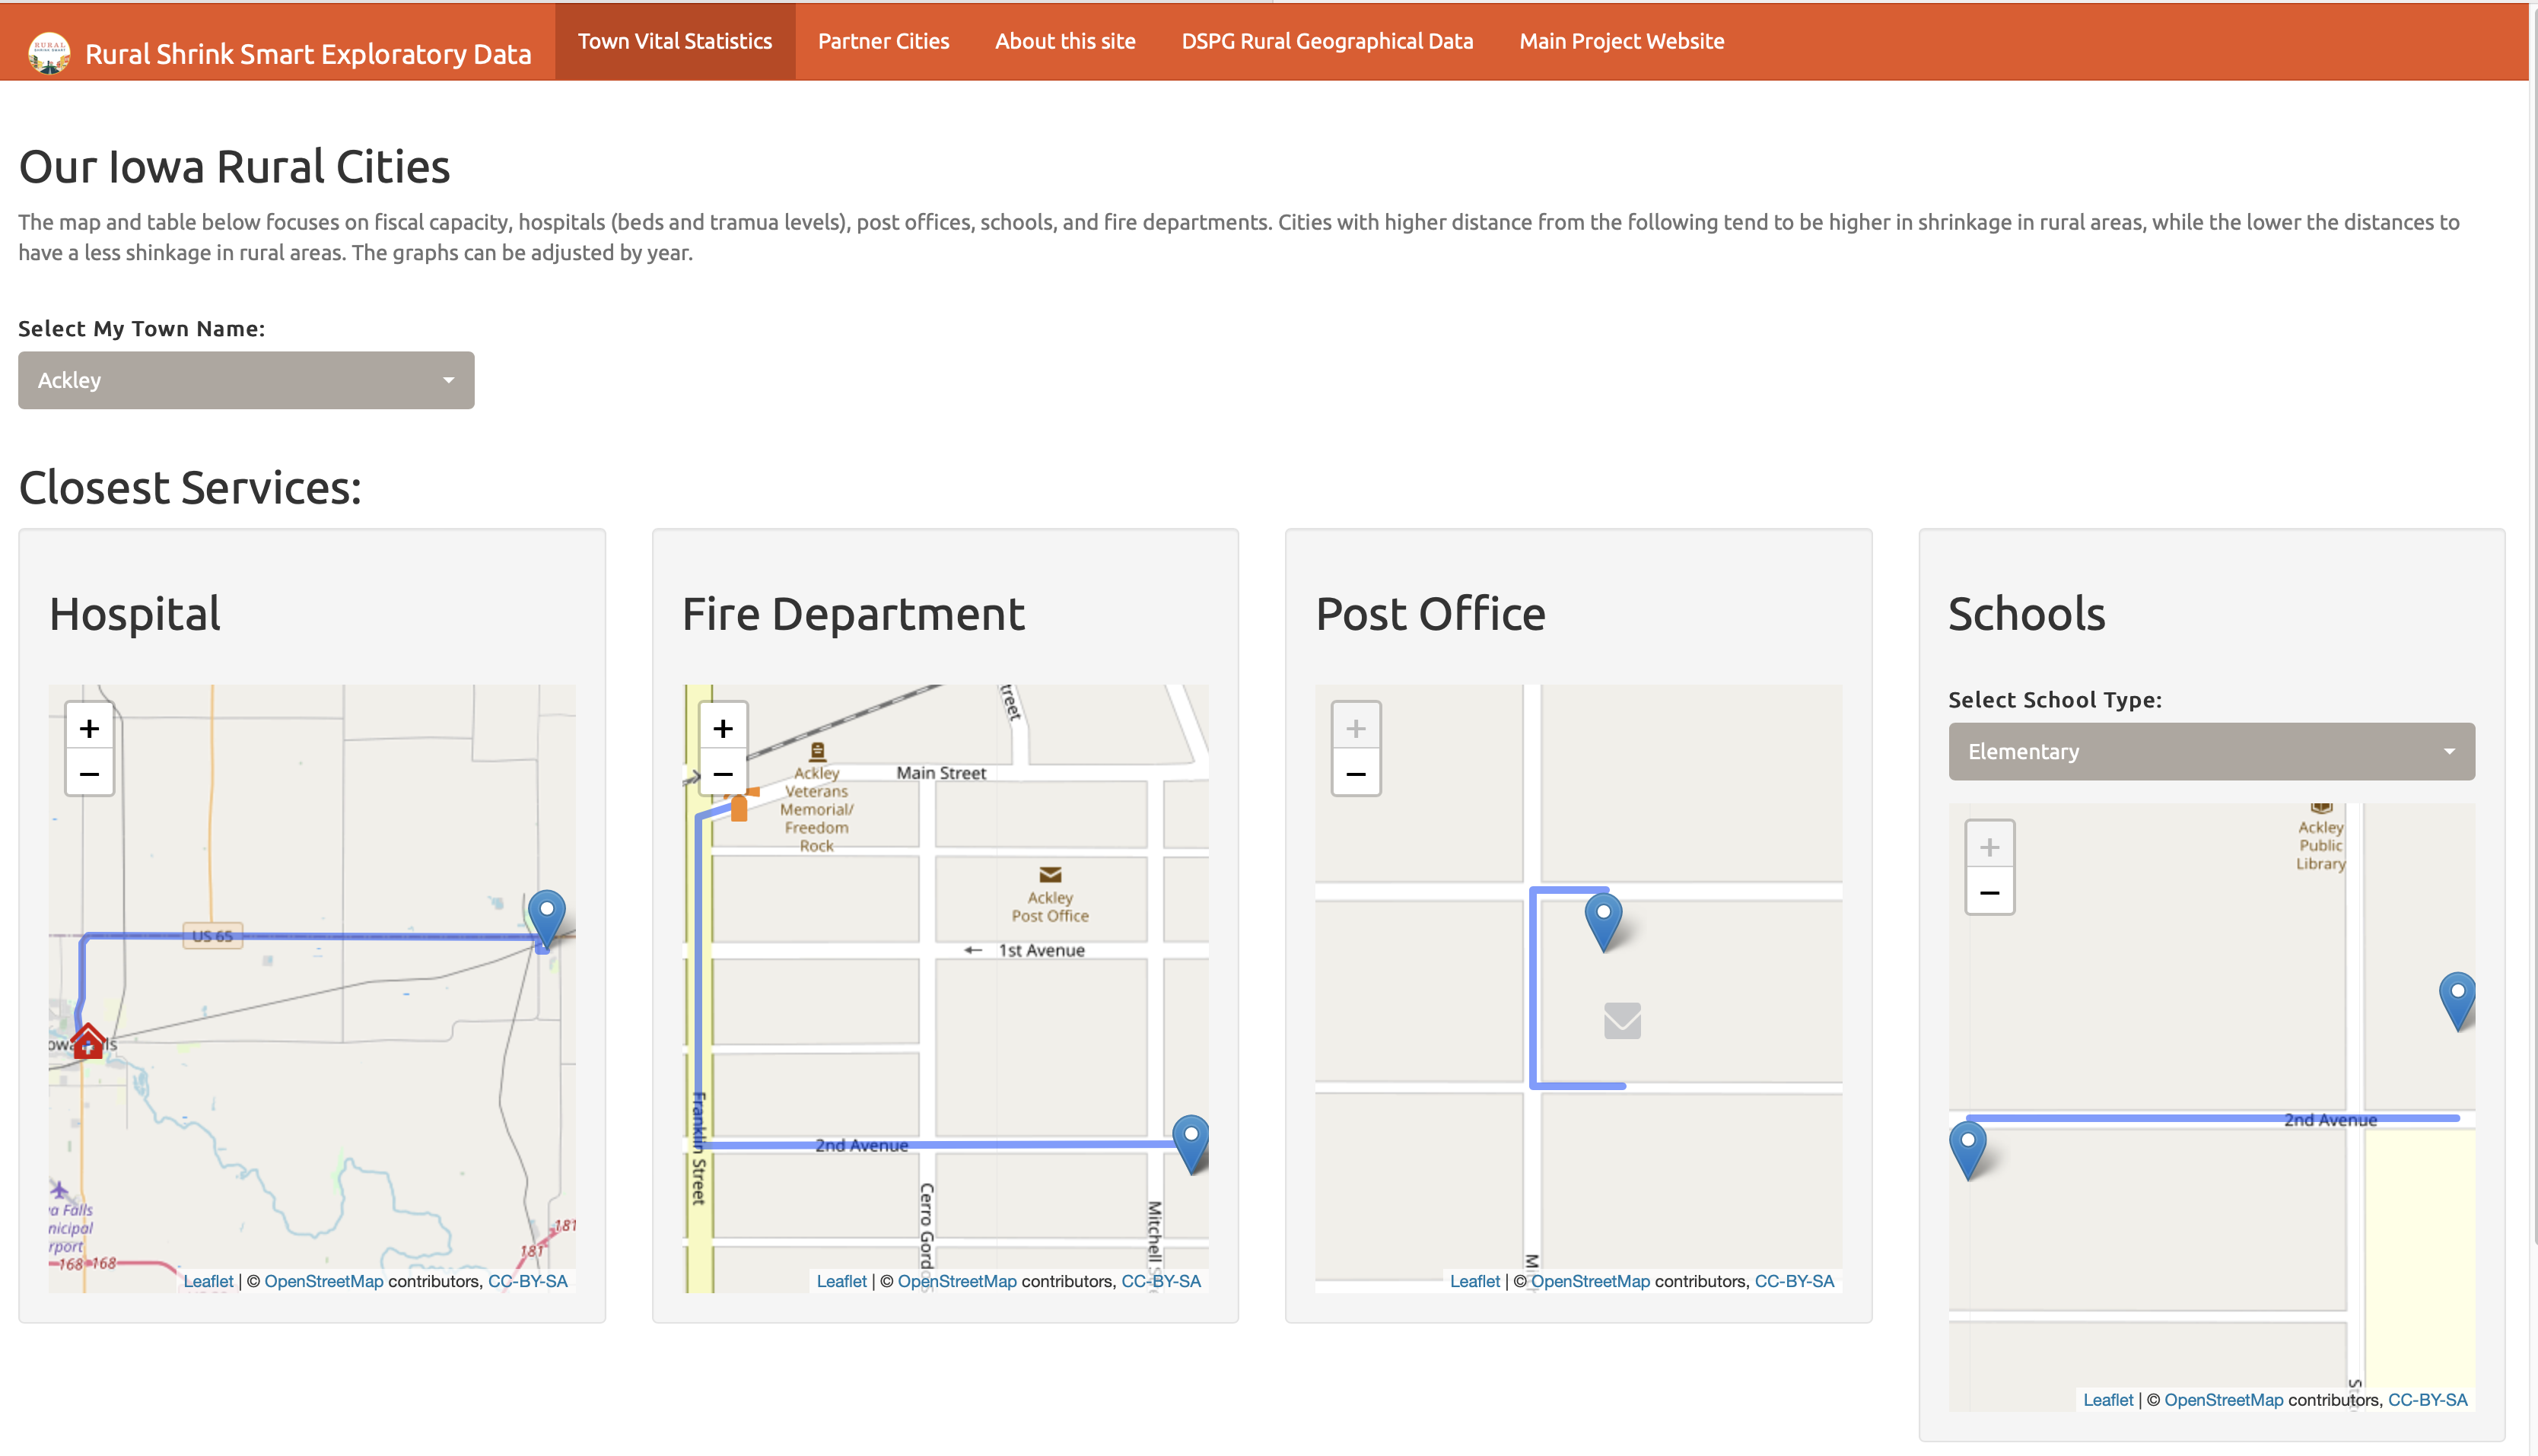
\includegraphics[width=75mm]{SCC_Dashboard.png}
\caption{Rural Smart EDA Dashboard Design}
\end{figure}


\subsection{Current Progress}
{\bf Statistical Techniques} Our research has incorporated statistical clustering methods, such as K-means and Hierarchical Clustering, to determine the similarities in the towns based on distances and services available. As a result, of our research partners we were actually able to use clustering methods to determine and identify missing data. We will continue to use clustering methods to identify the towns that will be best compare when the analyst interacts with our dashboard. 

{\bf Data Science Techniques} Our team has been able to utilize direct API calls and web scraping tools to collect data necessary.  

{\bf Dashboard Design Techniques} Our dashboard incorporates the following important dashboard techniques:
{\it User Flexibility} The aspects of user flexibility are directly based on the detail data adjustments; Adaptability: User and Display; Comparison support and Storytelling. For example, we want our users to use the data collected on a mass scale that have and should be summarized in detail but without losing anything.

{\it Visual, Analytic, and Data Literacy} The aspects in our dashboard development primary presents in our ability to ease of usage to the user with visual, data  and analytic literacy. We have little information on the users' adaptability to data-driven decisions. 

{\it Data Design}. In our case, the challenges that arise in our dashboard will include data quality, data grouping, too much data, data sources, inaccurate data representation, and key performance indicators and metrics. For example, we have information from {\it Iowa Data} will have missing data can be pointed out by our users' that has not been captured by our data sources, this can be a recent closing of a school due to the pandemic.

{\it Social Impact} This aspect will be about making sure that the users are flexible to the following: data-driven thinking, technology resistance, dashboard aversion, and data sharing, security, and privacy. For example, we will encounter town users that will have the urge to compare their town to all types of towns that aren't similar. In our research, we will use statistical clustering methods and cater dashboard to show only towns that have similar components.

\subsection{Future Work}
Our dashboard design has created challenges that promote 

We have five towns that have agreed to partner with the project to help with identify the best practices that are useful in the Iowa small and rural towns. As a result to our dashboard development, we will develop a feedback loop from the analyst in these five towns that will help provide our team with useful notes that will be adaptive to all of the small towns in Iowa. As a contrast, we will researchers with an extensive understanding of the small towns to be used as a counter example of dashboard adaptability. Our research, should be a 

So dashboard challenges,
adaptation techniques, and user strategies are interconnected as
Figure 1 shows. The rationale is that if we are able to establish
a relationship between strategies to problems and we can detect
the strategies in real-time, we can adapt the user interface in realtime or in the next iteration. Then we can say that the adaption
techniques have a positive effect on the challenges.
\section{Acknowledgements}
We would like to thank our sponsors and grant provider NSF, LSAMP Inspire Program and Iowa League of Cities. We would like to thank our partners and team members at Iowa State University and University of Nebraska - Lincoln. We would like to thank the State of Iowa for providing Data along with our partners in the Rural Iowa communities.


\bibliographystyle{sdss2020} % Please do not change the bibliography style
\bibliography{SCCAbstract_SDSS2022}

\end{document}
